\chapter{Preliminaries}\label{chapter:Preliminaries}

\section{Representation of Logic Circuits}
Independent of the underlying technology, digital circuits can be represented by logic functions. The Boolean Algebra, formed by mathematician George Boole in 1847, proposes these logic functions and provides a foundation to discuss about them.

\subsection{Boolean Functions}\label{subsec:boolfunc}
The definition as given here is based on an addition to Boolean calculus by Edward V. Huntington. CITE
The basis of a Boolean algebra is given as follows:

\begin{definition}[Basis for Boolean algebra]\label{Def:BasBool}
Given a finite set S, two binary functions · : S × S → S and + :
S × S → S, and one unary function ¬ : S → S, the tuple (S, ·,+,¬) is called a
Boolean algebra iff the following constraints hold for all a, b, c $\in$ S: \\

\centering
\begin{tabular}{l r l}

	     (1) & a · b = b · a & a + b = b + a \\

	     (2) &a · (b + c) = (a · b) + (a · c) & a + (b · c) = (a + b) · (a + c) \\
	     (3) & $\exists 1 \in S : a \cdot 1 = a$ &  $\exists 0 \in S : a + 0 = a$ \\
	     (4) &$\exists 0 \in S : a \cdot \neg a = 0$ & $\exists 1 \in S : a + \neg a = 1$. \\

\end{tabular}

\end{definition}

With the constraints describing (1) \textit{commutativity}, (2) \textit{distributivity}, (3) \textit{neutrality}, and (4)
\textit{complementarity}.\\

In the original definition a Boolean algebra is defined by the 6-tuple $(\mathbb{B}, \vee, \wedge, \neg, 0, 1)$, where $\vee$ and $\wedge$ are another denotations for the binary operands for disjunction $+$ and conjunction $\cdot$ in $\mathbb{B}$, the known unary negation function $\neg$, and two distinct elements 0 and 1. Negation $\neg a$ is also commonly notated as $\bar{a}$.\\

Since this definition is restricting the use of only the three Boolean functions $(\vee, \wedge, \neg)$, we want to extend by the following definition:

\begin{definition}
	A function $f : \mathbb{B}^n \to \mathbb{B}$, where $n \in N$, is called a Boolean function.
	Analogously, a
	function f : $\mathbb{B}^n \to \mathbb{B}^m$, where $n, m \in N$, is called multi-output Boolean function
	and can be interpreted as $f_v = (f_{v1}, . . . , f_{vm})$, where $f_{vi} : \mathbb{B}^n \to \mathbb{B}$, for all $1 \leq i \leq m$.
\end{definition}

A common notation for Boolean functions are the \textit{conjunctive normal form} (CNF) and \textit{disjunctive normal form} (DNF), using literals.

\begin{definition}
	A literal is an atom or the negation of an atom. In the former case the literal is positive, in the latter case it is negative.
\end{definition}

\begin{definition}
A formula F is in conjunctive normal form (CNF) if it is a
conjunction of disjunctions of literals:\\
\[\displaystyle\bigwedge_{i} \displaystyle\bigvee_{j} (\neg) v_{ij}, \]
where $v_{ij} \in \mathbb{B}$.\\
A formula F is in disjunctive normal form (DNF) if it is a
conjunction of disjunctions of literals:\\
\[ \displaystyle\bigvee_{i} \displaystyle\bigwedge_{j} (\neg) v_{ij}, \]
where $v_{ij} \in \mathbb{B}$.

\end{definition}

Using the CNF or rather the DNF and \textit{De Morgan's laws} following from the definitions in \ref{Def:BasBool}, it follows that any Boolean Algebra can be reduced to only two operands, e.g. conjunction ($\vee$) and negation ($\neg$). Any set of such two Boolean functions is called \textit{universal}.


\subsection{Logic Networks}

There are many ways of representing Boolean Functions. But most of them, including e.g. truth tables or reduced sum of products, suffer from drawbacks like exponential growth of size with the number of arguments and functions with exponential representations. The representation of combinational circuits as logic networks overcomes these restrictions and has proven to be very useful in the logic synthesis process. Following definition for directed acyclic graphs is shown in CITE:

\begin{definition}[Function graph]
	A function graph is a rooted, directed graph with vertex set $V$ containing two types of vertices. A \textit{nonterminal} vertex $v$ has as attributes an argument index $index(v) \in \{1, . . .,n\}$, and two children $low(v),high(v) \in V$. A \textit{terminal} vertex v has as attribute a value $value(v)\in\{0,1\}$.\\
	\\
	Furthermore, for any nonterminal vertex $v$, if $low(v)$ is also nonterminal, then we must have
	$index(v) < index(low(v))$. Similarly, if $high(v)$ is nonterminal, then we must have
	$index(v) < index(high(v))$.
\end{definition}

\begin{figure}
	\centering
	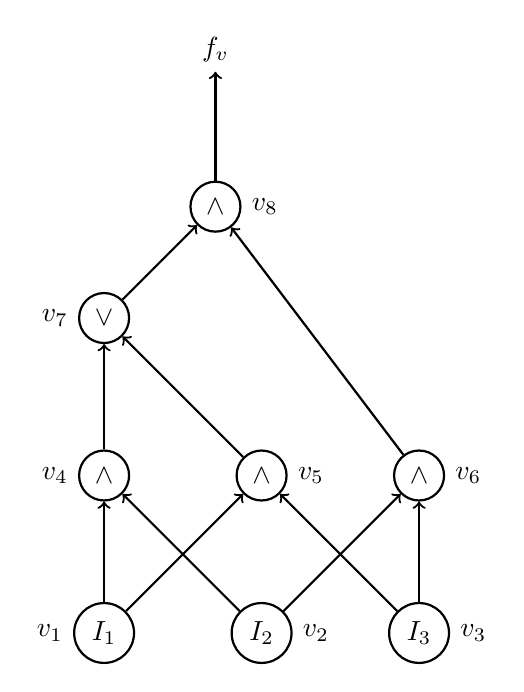
\begin{tikzpicture}[node distance={2cm and 2cm}, thick, main/.style = {draw, circle}] 
		\node[main] (1) [label=west:$v_1$]{$I_1$}; 
		\node[main] (2) [right of=1, label=east:$v_2$] {$I_2$};
		\node[main] (3) [right of=2, label=east:$v_3$] {$I_3$}; 
		
		\node[main] (4) [above of=1, label=west:$v_4$]{$\wedge$}; 
		\node[main] (5) [right of=4, label=east:$v_5$]{$\wedge$};
		\node[main] (6) [right of=5, label=east:$v_6$] {$\wedge$};
		
		\node[main] (7) [above of=4, label=west:$v_7$] {$\vee$};
		\node[main] (8) [above right of=7, label=east:$v_8$] {$\wedge$}; 
		\node [above of = 8] (f) {$f_v$};
		
		
		\draw[->] (1) -- (4);
		\draw[->] (1) -- (5);
		\draw[->] (2) -- (4);
		\draw[->] (2) -- (6);
		\draw[->] (3) -- (5);
		\draw[->] (3) -- (6);
		\draw[->] (4) -- (7);
		\draw[->] (5) -- (7);
		\draw[->] (7) -- (8);
		\draw[->] (6) -- (8);
		\draw[->] (8) -- (f);
		
	\end{tikzpicture} 
	\\
	\hfill \break
	The corresponding recursive Boolean functions read:\\
	\hfill \break
	\begin{tabular}{l l}
		
		$f_v = f_v(v_8)$ & $f_v(v_6) = f_v(v_2) \vee f_v(v_3)$ \\
		$f_v(v_8) = f_v(v_7) \wedge f_v(v_6)$ & $f_v(v_5) = f_v(v_3) \vee f_v(v_1)$ \\
		$f_v(v_7) = f_v(v_4) \wedge f_v(v_5)$ &  $f_v(v_4) = f_v(v_2) \vee f_v(v_1)$ \\
		&\\
		with primary inputs: & 	$f_v(v_1), f_v(v_2), f_v(v_3) \in \{0, 1\}$\\
		&\\
	\end{tabular}
	
	\caption{Binary Logic Network of Majority Function} \label{fig:LNMaj}
\end{figure}

Since the definition dosen't yet include Boolean Functions and reduces the number of children connected to a vertice to two, therefore only  allowing binary Boolean Functions, a custom definition is given:

\begin{definition}[Logic Network]
	A logic network is a rooted, directed graph with vertex set $V$ containing two types of vertices. A \textit{nonterminal} vertex $v$ has as attributes an argument index $index(v) \in \{1, . . .,n\}$, and $l$ children $child_1(v), ..., child_l(v) \in V$. A \textit{terminal} vertex v has as attribute a value $value(v)\in\{0,1\}$.\\
	\\
	Furthermore, for any nonterminal vertex $v$, if $child_i(v)$ with $ 1 \leq i \leq l$, then we must have
	$index(v) < index(child_i(v))$ respectively.
\end{definition}

\begin{definition}[Logic Network Boolean Functions]
	A set of nary Boolean Functions $\mathbb{B}$ is accessed via the argument index, assigning a Boolean Function $f_v$ to every vertex:
	\begin{enumerate}
		\item If v is a terminal vertex:
		\begin{enumerate}
			\item If $value(v)=1$, then $f_v=1$
			\item If $value(v)=0$, then $f_v=0$
		\end{enumerate}
		\item If $v$ is a nonterminal vertex with $index(v)=i$, then $f_v$ is the function \\ 
		$f_v(x_1, ..., x_n) = f_v(f_v(child_1(v)), ..., f_v(child_l(v)))$.
	\end{enumerate}
\end{definition}

The binary Logic Network of the ternary majority function is depicted figure \ref*{fig:LNMaj}:

\begin{definition}[Majority Function]\label{Def:majf}
	The ternary Boolean majority function is defined as: $<a, b, c> = ab + ac + bc$, so that the function value equals the majority of it's incoming values.\\
	It follows: $<a, b, 0> = ab$ and $<a, b, 1> = a + b$.
\end{definition}

Because of the names used in the underlying libraries used to program the algorithms proposed in chapter... the vertices are referred to as nodes, while edges connecting a vertex with one of its children is called a signal. Terminal vertices, found at the beginning of the graph and therefore possessing the lowest indices, are called primary inputs. The enumerated vertices $f_{vi}$, representing the boolean functions are called primary outputs.\\
!!ADD a Denotation\\
As already mentioned in subsection \ref{subsec:boolfunc}, a set of two certain Boolean functions can form any Boolean algebra.
As long as this universality is contained the set of node functions can be extended. Using conjunction and negation as the only node functions of a logic network, we get the so called \textit{AND-Inverter Graphs} (AIGs). Another widely used binary logic network is the \textit{Majority-Inverter Graphs} (MIGs) utilizing the ternary majority function and negation. But there also exists a wide range of logic networks permitting more than just two node functions, like \textit{XOR-AND-Inverter Graphs} (XAGs).\\

Since the logic network represents the combinational circuit in the given technology, a suitable logic network representation has to be determined. Because, even though these logic networks can implement any Boolean function given in a specification, not every logic network can be synthesized into any given technology.
Looking at the current standard technology \textit{complementary metal-oxidesemiconductor} (CMOS), the logic network is then synthesized by using building blocks consisting of \textit{metal-oxide-semiconductor field-effect transistors} (MOSFETs), the elemental unit in this technology. The process of turning a circuit specification into a logic gate representation is called \textit{logic synthesis}.\\

Given these logic network characteristics, none of the representations are \textit{canonical}, which means that a given function can be represented by different logic networks. This property can be explained by the fact that nodes with the identity function are allowed. Even the exclusion of such identity nodes has no impact, since simple node combinations, like two negotiation nodes, collapse to the identity function. Following this argumentation, there exists an infinite number of logic networks representing one Boolean Function, resulting in he widely accepted assumption, that the determination of an optimal logic network is a $\mathcal{NP}$-complete problem. Attempts to create canonical logic networks, seem to evade this problem, but include co$\mathcal{NP}$-complete problems in itself. Algorithms used for logic synthesis are therefore based on approximate solutions.


\section{QCA Technology}

Following the well known Moores law CMOS technology is facing a multitude of challenges, e.g. short channel effect, impurity variations, and most importantly the heat, resulting from static and dynamic power losses. To tackle these challenges the International Roadmap for Devices and Systems (IDRS), former ITRS, proposes solutions within the semiconductor domain, e.g. new materials and multi-core architectures. But also new technologies are researched including Quantum computing and the domain of \textit{Field-Coupled Nanocomputing} (FCN). This work focuses on one of the most promising FCN technologies, namely \textit{Quantum dot cellular automata} (QCA). The main difference of this technology compared to CMOS is the representation of logical modes, using the location of electron pairs in QCA-cells, instead of voltage levels. Data between cells is transferred based on Coulomb repulsion, utilizing electromagnetic fields. This enables the technology to achieve high performance in terms of device density, clock frequency and power consumption.

Point out why majority gates are a big part of this technology. \\
Point out why wires and especially wire crossings are so expensive to produce. \\

\subsection{Cells}
As already mentioned, the elemental unit of this technology is a QCA-cell. Since there in no uniform way of build the quantum dots and connecting them to cells, we look at a rather lower-level abstraction depicted in figure \ref{fig:QCAStates}. The four circles in the corners of the QCA-cells show quantum-dots, that can be implemented by any charge container with discrete electrical energy states. Further a cell contains two excess electrons, which can be localized by the quantum dots. The energy barriers or the quantum dots are able to trap the charge of the electron. If an electron is trapped inside a quantum-dot it is filled black. Due to the Coulomb repulsion the electrons occupy diagonally opposed quantum dots,
resulting in two possible stable cell configurations and one unstable cell configuration.\\
A stable states indicates, that it is well distinguishable of the usual energy band and therefore has a energy difference to another stable state of minimum the thermal noise energy ($k_BT$). Only such states are suited for information transfer. The stable states can be derived from the cell Polarization, which can be $+1$ and $-1$ or $null$ in the unexcited state. The two stable states contain the same electrostatic energy and are used to encode the binary values $0$ and $1$.\\
In order to transfer information, cells are placed side by side, whereby the polarization of the driver cell, which is the left most cell inputting the information, changes the polarization of the adjacent cell. When the adjacent cell is polarized it can give its state to the next cell and so on. This simple structure is representing a wire in QCA-technology and its function is depicted in Figure \ref{fig:QCAWire}.

\begin{figure}
	\centering
	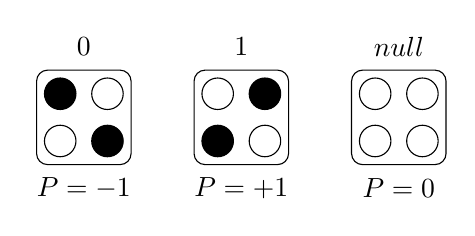
\begin{tikzpicture}
		%One QCA-Cell
		\node (A1) at (0.6,1.5) {$0$};
		\draw[rounded corners] (0, 0) rectangle (1.2, 1.2) [label=north:$v_7$]{};
		\node (A2) at (0.6,-0.3) {$P = -1$};
		
		\draw (0.3,0.3) circle (2mm);
		\draw [fill = black] (0.9,0.3) circle (2mm);
		\draw [fill = black](0.3,0.9) circle (2mm);
		\draw (0.9,0.9) circle (2mm);
		
		
		%One QCA-Cell
		\def\x{2}
		\node (B1) at (0.6+\x,1.5) {$1$};
		\draw[rounded corners] (\x, 0) rectangle (1.2 + \x, 1.2) {};
		\node (B2) at (0.6+\x,-0.3) {$P = +1$};
	
		\draw [fill = black] (0.3+\x,0.3) circle (2mm);
		\draw (0.9+\x,0.3) circle (2mm);
		\draw (0.3+\x,0.9) circle (2mm);
		\draw [fill = black] (0.9+\x,0.9) circle (2mm);
		
		
		%One QCA-Cell
		\def\x{4}
		\node (C1) at (0.6+\x,1.5) {$null$};
		\draw[rounded corners] (\x, 0) rectangle (1.2 + \x, 1.2) {};
		\node (C2) at (0.6+\x,-0.3) {$P = 0$};
		
		\draw (0.3+\x,0.3) circle (2mm);
		\draw (0.9+\x,0.3) circle (2mm);
		\draw (0.3+\x,0.9) circle (2mm);
		\draw (0.9+\x,0.9) circle (2mm);
		
		
	\end{tikzpicture} 

	\caption{QCA-Cell sates} \label{fig:QCAStates}
\end{figure}

\begin{figure}
	\centering
	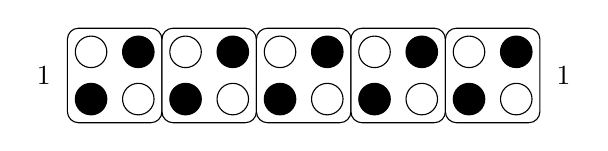
\begin{tikzpicture}
		%One QCA-Cell
		\node (A1) at (-0.3,0.6) {$1$};
		\draw[rounded corners] (0, 0) rectangle (1.2, 1.2) [label=north:$v_7$]{};
		
		\draw [fill = black](0.3,0.3) circle (2mm);
		\draw (0.9,0.3) circle (2mm);
		\draw (0.3,0.9) circle (2mm);
		\draw [fill = black](0.9,0.9) circle (2mm);
		
		
		%One QCA-Cell
		\def\x{1.2}
		\draw[rounded corners] (\x, 0) rectangle (1.2 + \x, 1.2) {};
		
		\draw [fill = black] (0.3+\x,0.3) circle (2mm);
		\draw (0.9+\x,0.3) circle (2mm);
		\draw (0.3+\x,0.9) circle (2mm);
		\draw [fill = black] (0.9+\x,0.9) circle (2mm);
		
		
		%One QCA-Cell
		\def\x{2.4}
		\draw[rounded corners] (\x, 0) rectangle (1.2 + \x, 1.2) {};
		\draw [fill = black](0.3+\x,0.3) circle (2mm);
		\draw (0.9+\x,0.3) circle (2mm);
		\draw (0.3+\x,0.9) circle (2mm);
		\draw [fill = black](0.9+\x,0.9) circle (2mm);
		
		%One QCA-Cell
		\def\x{3.6}
		\draw[rounded corners] (\x, 0) rectangle (1.2 + \x, 1.2) {};
		\draw [fill = black](0.3+\x,0.3) circle (2mm);
		\draw (0.9+\x,0.3) circle (2mm);
		\draw (0.3+\x,0.9) circle (2mm);
		\draw [fill = black](0.9+\x,0.9) circle (2mm);
		
		%One QCA-Cell
		\def\x{4.8}
		\draw[rounded corners] (\x, 0) rectangle (1.2 + \x, 1.2) {};
		\draw [fill = black](0.3+\x,0.3) circle (2mm);
		\draw (0.9+\x,0.3) circle (2mm);
		\draw (0.3+\x,0.9) circle (2mm);
		\draw [fill = black](0.9+\x,0.9) circle (2mm);
		\node (C1) at (1.5+\x,0.6) {$1$};
		
		
	\end{tikzpicture} 
	
	\caption{Adjacent QCA-cells forming a wire segment} \label{fig:QCAWire}
\end{figure}

\subsection{Information Transfer}\label{subsec:clocking}

As already mentioned the data transfer in the QCA paradigm is accomplished by cell-to-cell interaction. The leftmost cell has a fixed polarization and is called the input, while the right most cell represents the output of the simplified  QCA-circuit. Looking at the wire segment in figure \ref{fig:QCAWire}, we can see that in the ground state, all neighboring cells have the same polarization. This means that, with this given input, there exists exactly one configuration of cell polarization resulting in the minimum state energy of the wire. When the input of the system is changed, the systems energy rises, as depicted in figure \ref{fig:info_pass}. It results from the so called \textit{kink}-energy, which describes the energy difference between two QCA-cells with opposing polarization. In this state the \textit{kink} moves along the cells. While the \textit{kink}-energy stays the same, an increasing number of cells results in a rising degeneracy of the excited state. This again means, that the system is in an excited state at non-zero temperature. After time $\tau$ the system dissipates again into the ground state, with newly computed outputs.\\

The described process is called abrupt switching with dissipative coupling to the environment and can be summarized in the following three steps:
\begin{enumerate}
	\item Write the input bit by fixing the polarization state of
	cells along the input edge.
	\item Allow the array to relax to its ground state while the
	new inputs are kept fixed.
	\item Non-invasively read the results of the computation
	by sensing the polarization state of cells.
	%this is just copied
\end{enumerate}

In the second step, highly complex dissipation mechanisms like phonon and plasmon emission take place, making it nearly impossible to get a complete theoretical description of the system. The dissipation time $\tau$ is therefore determined via experiments.\\
The first and third step require an environment, which provides the features for fixing inputs and sensing the output polarization. Such a system has to be integrated with classical CMOS devices as seen in Figure \ref{fig:QCA_array}.\\

\begin{figure}
	\centering
	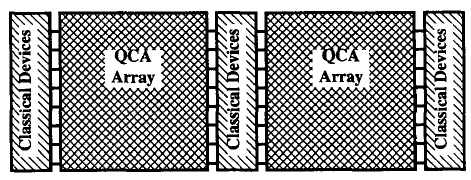
\includegraphics[scale=0.6]{QCA_array}
	\caption{Schematic of a combined QCA and CMOS sytem.} 
	\label{fig:QCA_array}
\end{figure}

\begin{figure}
	\centering
	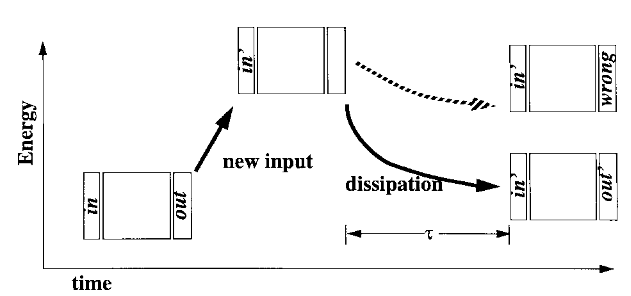
\includegraphics[scale=0.6]{information_passing}
	\caption{Schematic representation of a metastable state. Instead
		of relaxing correctly to the new ground state, a system may be
		delayed in an excited state due to an inability to tunnel through a
		kinetic barrier.} 
	\label{fig:info_pass}
\end{figure}

In order to implement a full QCA-system without CMOS-components, the QCA-Array has to be divided into smaller decoupled sub-regions. Therefore an adiabatic switching or rather a clocking is introduced. The clocked regions are referred to as clocking zones. The clocking utilizes an external signal, the clock, to activate and deactivate said clocking zones. The approach first used, decreases the interdot barriers of all cells in a clocking zone, when applying a new input. When all cells in the region are stable, the barriers are raised again, while the barriers of the subsequent clocking zone are lowered simultaneously. This way the ground state gradually propagates through the whole circuit. Today's used approaches create electrical fields with an external clock generator and distribute it to the cells through the device substrate using embedded electrodes. Thereby the energy level of the \textit{null} state can be controlled, resulting in a equivalent effect as in the former approach.\\

\begin{figure}
	\centering
	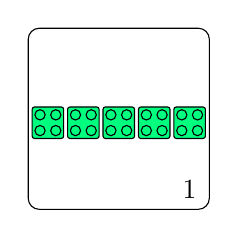
\begin{tikzpicture}
		\draw[rounded corners] (-0.05, -0.05 - 0.85) rectangle (2.3-0.05, 2.3-0.05 - 0.85){};
		\foreach \x/\xx in {0/0 ,0.4/0.05, 0.8/0.1, 1.2/0.15, 1.6/0.2}
		{
			
			\draw[rounded corners = 0.3mm, fill=SpringGreen] (\x + \xx, 0) rectangle (\xx + 1.2/3 + \x, 1.2/3){};
			\draw (0.3/3+ \x + \xx,0.3/3) circle (0.65mm);
			\draw (0.9/3+ \x + \xx,0.3/3) circle (0.65mm);
			\draw (0.3/3+ \x + \xx,0.9/3) circle (0.65mm);
			\draw (0.9/3+ \x + \xx,0.9/3) circle (0.65mm);
		}
		\node[text=black] (A1) at (2,-0.65) {$1$};
	\end{tikzpicture}%
	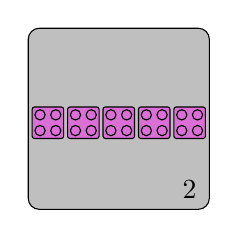
\begin{tikzpicture}
		\draw[rounded corners, fill=lightgray] (-0.05, -0.05 - 0.85) rectangle (2.3-0.05, 2.3-0.05 - 0.85){};
		\foreach \x/\xx in {0/0 ,0.4/0.05, 0.8/0.1, 1.2/0.15, 1.6/0.2}
		{
			
			\draw[rounded corners = 0.3mm, fill=Orchid] (\x + \xx, 0) rectangle (\xx + 1.2/3 + \x, 1.2/3){};
			\draw (0.3/3+ \x + \xx,0.3/3) circle (0.65mm);
			\draw (0.9/3+ \x + \xx,0.3/3) circle (0.65mm);
			\draw (0.3/3+ \x + \xx,0.9/3) circle (0.65mm);
			\draw (0.9/3+ \x + \xx,0.9/3) circle (0.65mm);
		}
		\node[text=black] (A1) at (2,-0.65) {$2$};
	\end{tikzpicture}%
	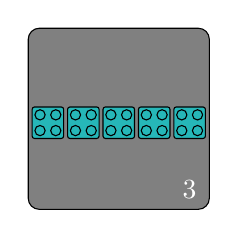
\begin{tikzpicture}
		\draw[rounded corners, fill=gray] (-0.05, -0.05 - 0.85) rectangle (2.3-0.05, 2.3-0.05 - 0.85){};
		\foreach \x/\xx in {0/0 ,0.4/0.05, 0.8/0.1, 1.2/0.15, 1.6/0.2}
		{
			
			\draw[rounded corners = 0.3mm, fill=BlueGreen] (\x + \xx, 0) rectangle (\xx + 1.2/3 + \x, 1.2/3){};
			\draw (0.3/3+ \x + \xx,0.3/3) circle (0.65mm);
			\draw (0.9/3+ \x + \xx,0.3/3) circle (0.65mm);
			\draw (0.3/3+ \x + \xx,0.9/3) circle (0.65mm);
			\draw (0.9/3+ \x + \xx,0.9/3) circle (0.65mm);
		}
		\node[text=white] (A1) at (2,-0.65) {$3$};
	\end{tikzpicture}%
	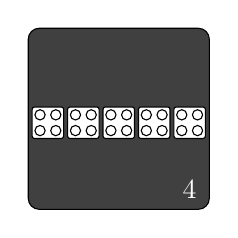
\begin{tikzpicture}
		\draw[rounded corners, fill=darkgray] (-0.05, -0.05 - 0.85) rectangle (2.3-0.05, 2.3-0.05 - 0.85){};
		\foreach \x/\xx in {0/0 ,0.4/0.05, 0.8/0.1, 1.2/0.15, 1.6/0.2}
		{
			
			\draw[rounded corners = 0.3mm, , fill=white] (\x + \xx, 0) rectangle (\xx + 1.2/3 + \x, 1.2/3){};
			\draw (0.3/3+ \x + \xx,0.3/3) circle (0.65mm);
			\draw (0.9/3+ \x + \xx,0.3/3) circle (0.65mm);
			\draw (0.3/3+ \x + \xx,0.9/3) circle (0.65mm);
			\draw (0.9/3+ \x + \xx,0.9/3) circle (0.65mm);
		}
		\node[text=white] (A1) at (2,-0.65) {$4$};
	\end{tikzpicture}%
	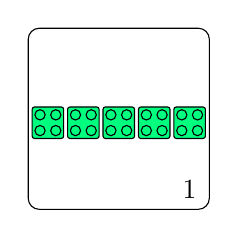
\begin{tikzpicture}
		\draw[rounded corners] (-0.05, -0.05 - 0.85) rectangle (2.3-0.05, 2.3-0.05 - 0.85){};
		\foreach \x/\xx in {0/0 ,0.4/0.05, 0.8/0.1, 1.2/0.15, 1.6/0.2}
		{
			
			\draw[rounded corners = 0.3mm, fill=SpringGreen] (\x + \xx, 0) rectangle (\xx + 1.2/3 + \x, 1.2/3){};
			\draw (0.3/3+ \x + \xx,0.3/3) circle (0.65mm);
			\draw (0.9/3+ \x + \xx,0.3/3) circle (0.65mm);
			\draw (0.3/3+ \x + \xx,0.9/3) circle (0.65mm);
			\draw (0.9/3+ \x + \xx,0.9/3) circle (0.65mm);
		}
		\node[text=black] (A1) at (2,-0.65) {$1$};
	\end{tikzpicture}%
	
	\caption{QCA-Cell wire with corresponding clock zones} \label{fig:QCAClock}
\end{figure}

A wire, divided in such clocking zones is shown in \ref{fig:QCAWire}. The colors of the zones and cells as well as the zone number show redundant information about the type of clocking zone. They differ in the external applied electrical field and therefore the energy of the cells. In QCA the clocking is divided into the four consecutive states, \textit{switch}, \textit{hold}, \textit{release} and \textit{relax}. They are aligned like in a pipeline like structure, where each of these state is phase shifted by $\pi/2$, forming a $2\pi$ clock cycle. In the switch-phase cells start getting polarized dependent on the polarization of the driving cell. When the cells are polarized they get fixed in the hold-phase. Afterwards in the release-phase the excitation gradually decreases, resulting in the unexcited relax-state. The scheme of such a pipeline like clocking is depicted exemplary on a wire segment in Figure \ref{fig:QCAClockpipeline}.

%%%%%%%%%%%%%%%%%%%%%%%%%%%%%%%%%%%%%%%%%%%%%%%%%%%%%%%%%%%%%

\begin{figure}
\tikzset{
	pics/cico/.style args={#1/#2/#3}{
		code = {
			\draw[rounded corners = 0.3mm] (#2 , #3) rectangle (1.2/3 + #2, 1.2/3 +#3){};
			\draw[fill = #1](0.3/3+ #2 ,0.3/3+ #3) circle (0.65mm);
			\draw (0.9/3+ #2 ,0.3/3+ #3) circle (0.65mm);
			\draw (0.3/3+ #2 ,0.9/3+ #3) circle (0.65mm);
			\draw[fill = #1] (0.9/3+ #2 ,0.9/3+ #3) circle (0.65mm);
}}}
	\centering
	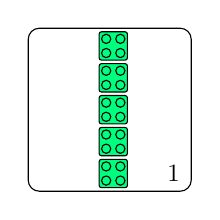
\begin{tikzpicture}[rotate=90, scale=0.9, every node/.style={scale=0.9}]
		\draw[rounded corners] (-0.05, -0.05 - 0.85) rectangle (2.3-0.05, 2.3-0.05 - 0.85){};
		\foreach \x/\xx in {0/0 ,0.4/0.05, 0.8/0.1, 1.2/0.15, 1.6/0.2}
		{
			
			\draw[rounded corners = 0.3mm, fill=SpringGreen] (\x + \xx, 0) rectangle (\xx + 1.2/3 + \x, 1.2/3){};
			\draw (0.3/3+ \x + \xx,0.3/3) circle (0.65mm);
			\draw (0.9/3+ \x + \xx,0.3/3) circle (0.65mm);
			\draw (0.3/3+ \x + \xx,0.9/3) circle (0.65mm);
			\draw (0.9/3+ \x + \xx,0.9/3) circle (0.65mm);
		}
		\node[text=black] (A1) at (0.2,-0.65) {$1$};
	\end{tikzpicture}
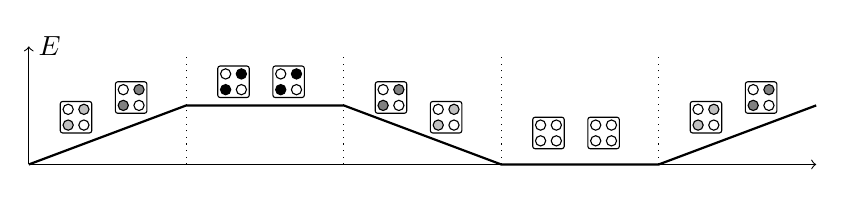
\begin{tikzpicture}
	
	% horizontal axis
	\draw[->] (0,0) -- (10,0) node[anchor=north] {};
	
	% vertical axis
	\draw[->] (0,0) -- (0,1.5) node[anchor=west] {$E$};
	% vertical lines
	\draw[dotted] (2,0) -- (2,1.4);
	\draw[dotted] (4,0) -- (4,1.4);
	\draw[dotted] (6,0) -- (6,1.4);
	\draw[dotted] (8,0) -- (8,1.4);
	
	% E
	\draw[thick] (0,0) -- (2,0.75) -- (4,0.75) -- (6,0) -- (8,0) --  (10,0.75);
	\draw (1,1.4) node {}; %label
	
	% Cells
	{
		\draw pic {cico=lightgray/0.4/0.4};		\draw pic {cico=gray/1.1/0.65};
		\draw pic {cico=black/2.4/0.85};		\draw pic {cico=black/3.1/0.85};
		\draw pic {cico=gray/4.4/0.65};			\draw pic {cico=lightgray/5.1/0.4};
		\draw pic {cico=white/6.4/0.2};			\draw pic {cico=white/7.1/0.2};
		\draw pic {cico=lightgray/8.4/0.4};		\draw pic {cico=gray/9.1/0.65};
	}
	
	
\end{tikzpicture}
\\
\vspace{-1.1pt}
	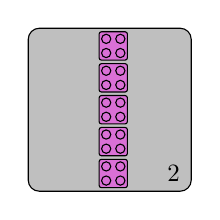
\begin{tikzpicture}[rotate=90, scale=0.9, every node/.style={scale=0.9}]
		\draw[rounded corners, fill=lightgray] (-0.05, -0.05 - 0.85) rectangle (2.3-0.05, 2.3-0.05 - 0.85){};
		\foreach \x/\xx in {0/0 ,0.4/0.05, 0.8/0.1, 1.2/0.15, 1.6/0.2}
		{
			
			\draw[rounded corners = 0.3mm, fill=Orchid] (\x + \xx, 0) rectangle (\xx + 1.2/3 + \x, 1.2/3){};
			\draw (0.3/3+ \x + \xx,0.3/3) circle (0.65mm);
			\draw (0.9/3+ \x + \xx,0.3/3) circle (0.65mm);
			\draw (0.3/3+ \x + \xx,0.9/3) circle (0.65mm);
			\draw (0.9/3+ \x + \xx,0.9/3) circle (0.65mm);
		}
		\node[text=black] (A1) at (0.2,-0.65) {$2$};
	\end{tikzpicture}
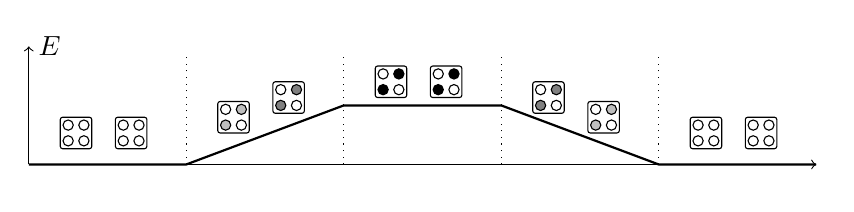
\begin{tikzpicture}
	
	% horizontal axis
	\draw[->] (0,0) -- (10,0) node[anchor=north] {};
	
	% vertical axis
	\draw[->] (0,0) -- (0,1.5) node[anchor=west] {$E$};
	% nominal speed
	\draw[dotted] (2,0) -- (2,1.4);
	\draw[dotted] (4,0) -- (4,1.4);
	\draw[dotted] (6,0) -- (6,1.4);
	\draw[dotted] (8,0) -- (8,1.4);
	
	% Us
	\draw[thick] (0,0) -- (2,0) -- (4,0.75) -- (6,0.75) -- (8,0) --  (10,0);
	\draw (1,1.4) node {}; %label
	
	% Cells

	{
		\draw pic {cico=white/0.4/0.2};			\draw pic {cico=white/1.1/0.2};
		\draw pic {cico=lightgray/2.4/0.4};		\draw pic {cico=gray/3.1/0.65};
		\draw pic {cico=black/4.4/0.85};		\draw pic {cico=black/5.1/0.85};
		\draw pic {cico=gray/6.4/0.65};			\draw pic {cico=lightgray/7.1/0.4};
		\draw pic {cico=white/8.4/0.2};			\draw pic {cico=white/9.1/0.2};
	}
	
	
\end{tikzpicture}
\\
\vspace{-1.1pt}
	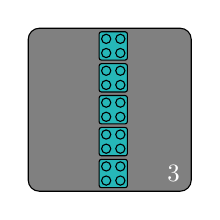
\begin{tikzpicture}[rotate=90, scale=0.9, every node/.style={scale=0.9}]
		\draw[rounded corners, fill=gray] (-0.05, -0.05 - 0.85) rectangle (2.3-0.05, 2.3-0.05 - 0.85){};
		\foreach \x/\xx in {0/0 ,0.4/0.05, 0.8/0.1, 1.2/0.15, 1.6/0.2}
		{
			
			\draw[rounded corners = 0.3mm, fill=BlueGreen] (\x + \xx, 0) rectangle (\xx + 1.2/3 + \x, 1.2/3){};
			\draw (0.3/3+ \x + \xx,0.3/3) circle (0.65mm);
			\draw (0.9/3+ \x + \xx,0.3/3) circle (0.65mm);
			\draw (0.3/3+ \x + \xx,0.9/3) circle (0.65mm);
			\draw (0.9/3+ \x + \xx,0.9/3) circle (0.65mm);
		}
		\node[text=white] (A1) at (0.2,-0.65) {$3$};
	\end{tikzpicture}
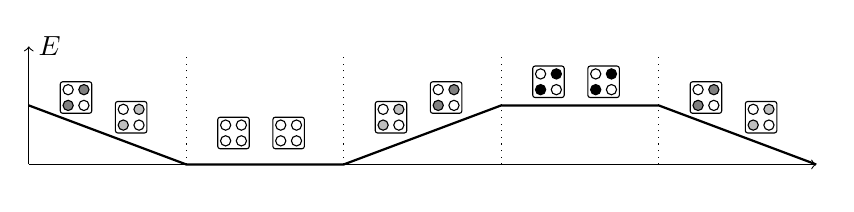
\begin{tikzpicture}
	
	% horizontal axis
	\draw[->] (0,0) -- (10,0) node[anchor=north] {};
	
	% vertical axis
	\draw[->] (0,0) -- (0,1.5) node[anchor=west] {$E$};
	% nominal speed
	\draw[dotted] (2,0) -- (2,1.4);
	\draw[dotted] (4,0) -- (4,1.4);
	\draw[dotted] (6,0) -- (6,1.4);
	\draw[dotted] (8,0) -- (8,1.4);
	
	% Us
	\draw[thick] (0,0.75) -- (2,0) -- (4,0) -- (6,0.75) -- (8,0.75) --  (10,0);
	\draw (1,1.4) node {}; %label
	
	% Cells
	{
		\draw pic {cico=gray/0.4/0.65};			\draw pic {cico=lightgray/1.1/0.4};
		\draw pic {cico=white/2.4/0.2};			\draw pic {cico=white/3.1/0.2};
		\draw pic {cico=lightgray/4.4/0.4};		\draw pic {cico=gray/5.1/0.65};
		\draw pic {cico=black/6.4/0.85};		\draw pic {cico=black/7.1/0.85};
		\draw pic {cico=gray/8.4/0.65};			\draw pic {cico=lightgray/9.1/0.4};
	}
	
	
\end{tikzpicture}
\\
\vspace{-1.1pt}
	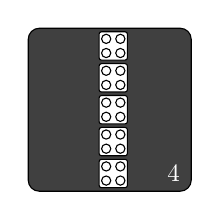
\begin{tikzpicture}[rotate=90, scale=0.9, every node/.style={scale=0.9}]
		\draw[rounded corners, fill=darkgray] (-0.05, -0.05 - 0.85) rectangle (2.3-0.05, 2.3-0.05 - 0.85){};
		\foreach \x/\xx in {0/0 ,0.4/0.05, 0.8/0.1, 1.2/0.15, 1.6/0.2}
		{
			
			\draw[rounded corners = 0.3mm, , fill=white] (\x + \xx, 0) rectangle (\xx + 1.2/3 + \x, 1.2/3){};
			\draw (0.3/3+ \x + \xx,0.3/3) circle (0.65mm);
			\draw (0.9/3+ \x + \xx,0.3/3) circle (0.65mm);
			\draw (0.3/3+ \x + \xx,0.9/3) circle (0.65mm);
			\draw (0.9/3+ \x + \xx,0.9/3) circle (0.65mm);
		}
		\node[text=white] (A1) at (0.2,-0.65) {$4$};
	\end{tikzpicture}
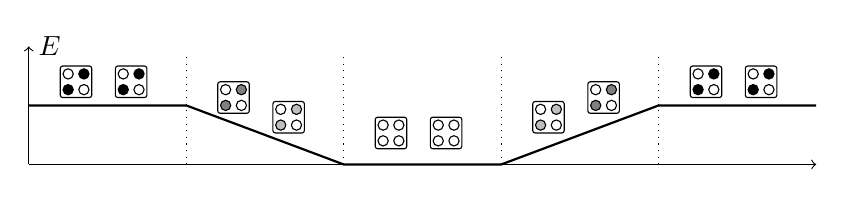
\begin{tikzpicture}
	
	% horizontal axis
	\draw[->] (0,0) -- (10,0) node[anchor=north] {};
	
	% vertical axis
	\draw[->] (0,0) -- (0,1.5) node[anchor=west] {$E$};
	% nominal speed
	\draw[dotted] (2,0) -- (2,1.4);
	\draw[dotted] (4,0) -- (4,1.4);
	\draw[dotted] (6,0) -- (6,1.4);
	\draw[dotted] (8,0) -- (8,1.4);
	
	% Us
	\draw[thick] (0,0.75) -- (2,0.75) -- (4,0) -- (6,0) -- (8,0.75) --  (10,0.75);
	\draw (1,1.4) node {}; %label
	
	% Cells
	
	{
		\draw pic {cico=black/0.4/0.85};		\draw pic {cico=black/1.1/0.85};
		\draw pic {cico=gray/2.4/0.65};			\draw pic {cico=lightgray/3.1/0.4};
		\draw pic {cico=white/4.4/0.2};			\draw pic {cico=white/5.1/0.2};
		\draw pic {cico=lightgray/6.4/0.4};		\draw pic {cico=gray/7.1/0.65};
		\draw pic {cico=black/8.4/0.85};		\draw pic {cico=black/9.1/0.85};
	}
	
	
\end{tikzpicture}
	\caption{QCA clocking pipeline} \label{fig:QCAClockpipeline}
\end{figure}


The described clocking is named \textit{Landauer clocking}. The inventor Rolf Landauer himself pointed out the vast power dissipation of this clocking mechanism. This impairing property is already well known from the CMOS technology, resulting in several drawbacks including switched off chip areas referred to as dark silicon in extreme cases. One common approach is the lowering of circuit frequency utilizing e.g. multi-chip architectures. To tackle this problem in the QCA domain, Landauer pointed out that the \textit{erase} function has to be eliminated from the clocking. This function is logically irreversible and describes the erasing of information in a clock zone, when passed to the next. He argued that every erased bit dissipates at least $k_BT\ln(2)$ in heat. Exemplary if a QCA-cell has size $1nm \times 1nm$ and operating frequency of $100 GHz$, the corresponding density of devices results to $10^{14}$ $cm^{-2}$. Further a dissipation of $0.1 eV$ per electron every clock cycle is assumed, resulting in a total power dissipation of 160 $kW$ $cm^{-2}$. This directly yields to the statement, that a device operating with this clocking would be inoperable (it would evaporate due to the heat). The \textit{Bennet clocking} tackles exactly this problem by altering the timing of the clocking signals. Just as in the Landau clocking the clocking-wave moves from left to right, but leaving no trailing edge, when information is passed. Instead the cells will be held in the excited state until the information propagates through the whole QCA-array. When the output was read, the excitation is released in reverse order resulting in no erase functions. This means, that this \textit{quasi-adiabatic} clocking leads to a minimal power dissipation but with two constraints. The effective clock rate is at least halved due to the additional backwards propagation and since only one signal vector can be transmitted through the system, the pipeline capabilities are reduced.\\
As already stated the QCA-array has to be divided into clock zones. Allowing an arbitrary number of cells in one clock zone allows lots of freedom for the clocking and is called \textit{cell-based} clocking. This freedom leads to clock zones with variable geometries, which again lead to variation in their fabrication. Assuming the necessity of an uniform fabrication to fabricate circuits with millions of cells, this clocking gets infeasible for large circuits. Also the scheme supports clocking of single cells, which means that electrodes of the same size have to be fabricated. Since this is also not feasible, this design is obsolete.\\ 
In order to attain uniform clocking zones with a possible distribution of clocking signals, the \textit{tile-based} clocking is introduced. The approach of this design is to provide uniform square tiles of the size $3 \times 3$ or $5 \times 5$. For clocking tiles bigger than this, the information propagation was suggested to be erroneous, also following in an argument against cell-based clocking.


\begin{figure}
	\newcommand*{\xMin}{0}%
	\newcommand*{\xMax}{4}%
	\newcommand*{\xMaxc}{3}%
	\newcommand*{\yMin}{0}%
	\newcommand*{\yMax}{4}%
	\newcommand*{\yMaxc}{3}%
	\subfigure[2DDWave]
	{
		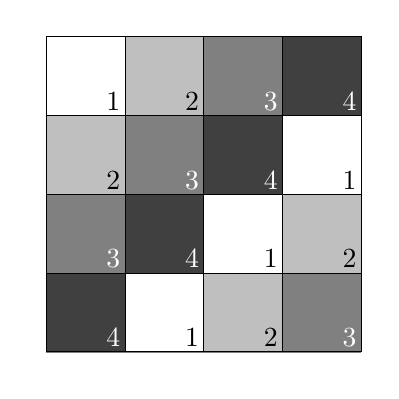
\begin{tikzpicture}
			
			\foreach \i in {\xMin,...,\xMax} {
				\draw [very thin,gray] (\i,\yMin) -- (\i,\yMax)  node [below] at (\i,\yMin) {};
			}
			\foreach \i in {\yMin,...,\yMax} {
				\draw [very thin,gray] (\xMin,\i) -- (\xMax,\i) node [left] at (\xMin,\i) {};
			}
		
		
			\draw[fill=darkgray]  (0, 1) -- (1, 1) -- (1,0) -- (0,0) -- cycle;
			\draw[fill=white]  (1, 1) -- (2, 1) -- (2,0) -- (1,0) -- cycle;
			\draw[fill=lightgray]  (2, 1) -- (3, 1) -- (3,0) -- (2,0) -- cycle;
			\draw[fill=gray]  (3, 1) -- (4, 1) -- (4,0) -- (3,0) -- cycle;
			
			\draw[fill=gray]  (0, 2) -- (1, 2) -- (1,1) -- (0,1) -- cycle;
			\draw[fill=darkgray]  (1, 2) -- (2, 2) -- (2,1) -- (1,1) -- cycle;
			\draw[fill=white]  (2, 2) -- (3, 2) -- (3,1) -- (2,1) -- cycle;
			\draw[fill=lightgray]  (3, 2) -- (4, 2) -- (4,1) -- (3,1) -- cycle;
			
			\draw[fill=lightgray]  (0, 3) -- (1, 3) -- (1,2) -- (0,2) -- cycle;
			\draw[fill=gray]  (1, 3) -- (2, 3) -- (2,2) -- (1,2) -- cycle;
			\draw[fill=darkgray]  (2, 3) -- (3, 3) -- (3,2) -- (2,2) -- cycle;
			\draw[fill=white]  (3, 3) -- (4, 3) -- (4,2) -- (3,2) -- cycle;
			
			\draw[fill=white]  (0, 4) -- (1, 4) -- (1,3) -- (0,3) -- cycle;
			\draw[fill=lightgray]  (1, 4) -- (2, 4) -- (2,3) -- (1,3) -- cycle;
			\draw[fill=gray]  (2, 4) -- (3, 4) -- (3,3) -- (2,3) -- cycle;
			\draw[fill=darkgray]  (3, 4) -- (4, 4) -- (4,3) -- (3,3) -- cycle;
			
			\node[text=white] (A1) at (0.85,0.18) {$4$};
			\node[text=black] (A1) at (1.85,0.18) {$1$};
			\node[text=black] (A1) at (2.85,0.18) {$2$};
			\node[text=white] (A1) at (3.85,0.18) {$3$};
			
			\node[text=white] (A1) at (0.85,1.18) {$3$};
			\node[text=white] (A1) at (1.85,1.18) {$4$};
			\node[text=black] (A1) at (2.85,1.18) {$1$};
			\node[text=black] (A1) at (3.85,1.18) {$2$};
			
			\node[text=black] (A1) at (0.85,2.18) {$2$};
			\node[text=white] (A1) at (1.85,2.18) {$3$};
			\node[text=white] (A1) at (2.85,2.18) {$4$};
			\node[text=black] (A1) at (3.85,2.18) {$1$};
			
			\node[text=black] (A1) at (0.85,3.18) {$1$};
			\node[text=black] (A1) at (1.85,3.18) {$2$};
			\node[text=white] (A1) at (2.85,3.18) {$3$};
			\node[text=white] (A1) at (3.85,3.18) {$4$};
	
		
		\end{tikzpicture}
	\label{subfig:2DD}
	}
	\subfigure[USE]
	{
		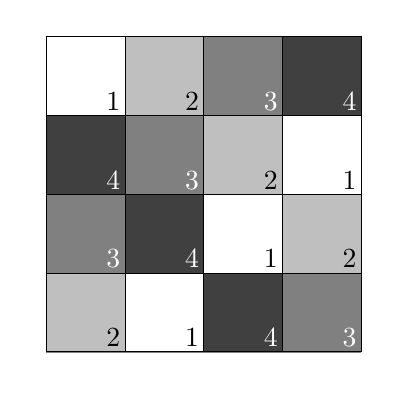
\begin{tikzpicture}
			\foreach \i in {\xMin,...,\xMax} {
				\draw [very thin,gray] (\i,\yMin) -- (\i,\yMax)  node [below] at (\i,\yMin) {};
			}
			\foreach \i in {\yMin,...,\yMax} {
				\draw [very thin,gray] (\xMin,\i) -- (\xMax,\i)
				node [left] at (\xMin,\i) {};
			}
		\draw[fill=lightgray]  (0, 1) -- (1, 1) -- (1,0) -- (0,0) -- cycle;
		\draw[fill=white]  (1, 1) -- (2, 1) -- (2,0) -- (1,0) -- cycle;
		\draw[fill=darkgray]  (2, 1) -- (3, 1) -- (3,0) -- (2,0) -- cycle;
		\draw[fill=gray]  (3, 1) -- (4, 1) -- (4,0) -- (3,0) -- cycle;
		
		\draw[fill=gray]  (0, 2) -- (1, 2) -- (1,1) -- (0,1) -- cycle;
		\draw[fill=darkgray]  (1, 2) -- (2, 2) -- (2,1) -- (1,1) -- cycle;
		\draw[fill=white]  (2, 2) -- (3, 2) -- (3,1) -- (2,1) -- cycle;
		\draw[fill=lightgray]  (3, 2) -- (4, 2) -- (4,1) -- (3,1) -- cycle;
		
		\draw[fill=darkgray]  (0, 3) -- (1, 3) -- (1,2) -- (0,2) -- cycle;
		\draw[fill=gray]  (1, 3) -- (2, 3) -- (2,2) -- (1,2) -- cycle;
		\draw[fill=lightgray]  (2, 3) -- (3, 3) -- (3,2) -- (2,2) -- cycle;
		\draw[fill=white]  (3, 3) -- (4, 3) -- (4,2) -- (3,2) -- cycle;
		
		\draw[fill=white]  (0, 4) -- (1, 4) -- (1,3) -- (0,3) -- cycle;
		\draw[fill=lightgray]  (1, 4) -- (2, 4) -- (2,3) -- (1,3) -- cycle;
		\draw[fill=gray]  (2, 4) -- (3, 4) -- (3,3) -- (2,3) -- cycle;
		\draw[fill=darkgray]  (3, 4) -- (4, 4) -- (4,3) -- (3,3) -- cycle;
		
		\node[text=black] (A1) at (0.85,0.18) {$2$};
		\node[text=black] (A1) at (1.85,0.18) {$1$};
		\node[text=white] (A1) at (2.85,0.18) {$4$};
		\node[text=white] (A1) at (3.85,0.18) {$3$};
		
		\node[text=white] (A1) at (0.85,1.18) {$3$};
		\node[text=white] (A1) at (1.85,1.18) {$4$};
		\node[text=black] (A1) at (2.85,1.18) {$1$};
		\node[text=black] (A1) at (3.85,1.18) {$2$};
		
		\node[text=white] (A1) at (0.85,2.18) {$4$};
		\node[text=white] (A1) at (1.85,2.18) {$3$};
		\node[text=black] (A1) at (2.85,2.18) {$2$};
		\node[text=black] (A1) at (3.85,2.18) {$1$};
		
		\node[text=black] (A1) at (0.85,3.18) {$1$};
		\node[text=black] (A1) at (1.85,3.18) {$2$};
		\node[text=white] (A1) at (2.85,3.18) {$3$};
		\node[text=white] (A1) at (3.85,3.18) {$4$};
		\end{tikzpicture}
	\label{subfig:USE}
	}
	\subfigure[RES]
	{
		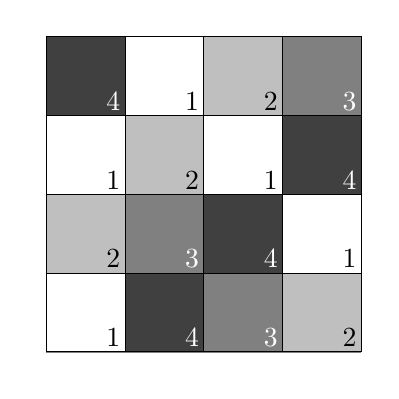
\begin{tikzpicture}
			\foreach \i in {\xMin,...,\xMax} {
				\draw [very thin,gray] (\i,\yMin) -- (\i,\yMax)
				node [below] at (\i,\yMin) {};
			}
			\foreach \i in {\yMin,...,\yMax} {
				\draw [very thin,gray] (\xMin,\i) -- (\xMax,\i)
				node [left] at (\xMin,\i) {};
			}
		\draw[fill=white]  (0, 1) -- (1, 1) -- (1,0) -- (0,0) -- cycle;
		\draw[fill=darkgray]  (1, 1) -- (2, 1) -- (2,0) -- (1,0) -- cycle;
		\draw[fill=gray]  (2, 1) -- (3, 1) -- (3,0) -- (2,0) -- cycle;
		\draw[fill=lightgray]  (3, 1) -- (4, 1) -- (4,0) -- (3,0) -- cycle;
		
		\draw[fill=lightgray]  (0, 2) -- (1, 2) -- (1,1) -- (0,1) -- cycle;
		\draw[fill=gray]  (1, 2) -- (2, 2) -- (2,1) -- (1,1) -- cycle;
		\draw[fill=darkgray]  (2, 2) -- (3, 2) -- (3,1) -- (2,1) -- cycle;
		\draw[fill=white]  (3, 2) -- (4, 2) -- (4,1) -- (3,1) -- cycle;
		
		\draw[fill=white]  (0, 3) -- (1, 3) -- (1,2) -- (0,2) -- cycle;
		\draw[fill=lightgray]  (1, 3) -- (2, 3) -- (2,2) -- (1,2) -- cycle;
		\draw[fill=white]  (2, 3) -- (3, 3) -- (3,2) -- (2,2) -- cycle;
		\draw[fill=darkgray]  (3, 3) -- (4, 3) -- (4,2) -- (3,2) -- cycle;
		
		\draw[fill=darkgray]  (0, 4) -- (1, 4) -- (1,3) -- (0,3) -- cycle;
		\draw[fill=white]  (1, 4) -- (2, 4) -- (2,3) -- (1,3) -- cycle;
		\draw[fill=lightgray]  (2, 4) -- (3, 4) -- (3,3) -- (2,3) -- cycle;
		\draw[fill=gray]  (3, 4) -- (4, 4) -- (4,3) -- (3,3) -- cycle;
		
		\node[text=black] (A1) at (0.85,0.18) {$1$};
		\node[text=white] (A1) at (1.85,0.18) {$4$};
		\node[text=white] (A1) at (2.85,0.18) {$3$};
		\node[text=black] (A1) at (3.85,0.18) {$2$};
		
		\node[text=black] (A1) at (0.85,1.18) {$2$};
		\node[text=white] (A1) at (1.85,1.18) {$3$};
		\node[text=white] (A1) at (2.85,1.18) {$4$};
		\node[text=black] (A1) at (3.85,1.18) {$1$};
		
		\node[text=black] (A1) at (0.85,2.18) {$1$};
		\node[text=black] (A1) at (1.85,2.18) {$2$};
		\node[text=black] (A1) at (2.85,2.18) {$1$};
		\node[text=white] (A1) at (3.85,2.18) {$4$};
		
		\node[text=white] (A1) at (0.85,3.18) {$4$};
		\node[text=black] (A1) at (1.85,3.18) {$1$};
		\node[text=black] (A1) at (2.85,3.18) {$2$};
		\node[text=white] (A1) at (3.85,3.18) {$3$};
		\end{tikzpicture}
	\label{subfig:RES}
	}
	
	\caption{Different clocking Schemes in QCA} \label{fig:ClockingSchemes}
\end{figure}

The tile-based clocking leads to several proposals of clocking-schemes, which give a certain distribution of clock zones. Since they follow an uniform pattern they can be extended easily for every size of the circuit. In \ref{fig:ClockingSchemes} three clocking schemes are showed, each of them based on a different idea. Since information is only allowed in ascending clock order (except 4 to 1), the 2DDWave clocking scheme in figure \ref{subfig:2DD} only allows information to propagate in two directions, south and north. This simplicity allows no back propagation, prohibiting the placement of sequential circuits. Also it restricts gates in the scheme to have a maximum input size of two. The USE scheme \ref{subfig:USE} tackles the first problem by introducing clocking loops into the scheme, giving the possibility to place sequential circuits. To tackle the second problem, the RES scheme \ref{subfig:RES} gives an opportunity to place gates of input size three. Since one tile is restricted to four adjacent cells of which one has to output the information of the cell, this gives the maximum input size allowed. This is especially important for the placement of majority-gates. In QCA-technology they can be represented by only one tile, making it to a huge advantage over CMOS technology. This is further evaluated in the next subsection on gates.

\subsection{Gates}\label{sub:gates}

\begin{figure}
	\centering
	
	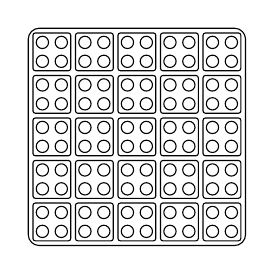
\begin{tikzpicture}[rotate=90, scale=1.2, every node/.style={scale=1.2}]
		\draw[rounded corners] (-0.05, -0.1 - 0.85) rectangle (2.3-0.05, 2.3-0.1 - 0.85){};
		
		\foreach \y in {-0.45, -0.9, 0, 0.45, 0.9}
		{
			\foreach \x in {0 ,0.45, 0.9, 1.35, 1.8}
			{
				
				\draw[rounded corners = 0.3mm] (\x, 0 + \y) rectangle (1.2/3 + \x, 1.2/3 + \y){};
				\draw (0.3/3+ \x,0.3/3 + \y) circle (0.65mm);
				\draw (0.9/3+ \x,0.3/3+ \y) circle (0.65mm);
				\draw (0.3/3+ \x,0.9/3 + \y) circle (0.65mm);
				\draw (0.9/3+ \x,0.9/3 + \y) circle (0.65mm);
			}
		}
	\end{tikzpicture}
	
	\label{fig:Celltile}\caption{Cell representation of tile}
\end{figure}
In this chapter a library of gates is introduced, which are later used in the proposed placement and routing algorithms. In \cite{QCA_scl} a custom QCA library called QCA ONE is proposed. It contains gates formed by both one and multiple tiles. A major drawback of this library is the prerequisite of a clocking scheme in order to form multiple tile gates. This restricts the underlying placement and routing algorithm to this exact clocking scheme. Also manual changes of the standard cells clock zones, size or positioning is not allowed, imposing the designer with even more restrictions. The standard cell library used for this work should only contain gates occupying one tile. Every other gate is composed out of these standard cells. The tiles used are of the dimension $5 \times 5$, which means that all standard gates are reduced to this area.\\
The first gate in the library is the inverter or NOT gate. The simplest implementation is shown in figure !!. It consists of two wire segments which are shifted by exactly one cell height, so that the polarization is transferred diagonally resulting in an inversion of the input. In order to get a more robust gate regarding disturbance, the C-shaped inverter shown in figure !! is introduced. This gate is used as standard in many libraries and works !! but it still has to be mentioned that this implementation is really prone to common displacement faults \cite{Inverter_displacements}, suggesting the addition of an inverter leg resulting to a E-shaped gate structure, and more complex single electron faults \cite{SingelElectronFaults}. Nevertheless the C-shaped inverter gate is selected as standard cell for this work.\\
The most important gate in QCA technology is the majority gate. To implement this function in CMOS technology after Definition \ref{Def:majf} multiple AND and OR gates have to be used. In QCA technology the majority function can be represented by exactly one gate, making it one of the major advantages over CMOS technology. There are two main implementations of the majority gate. The rotated majority gate in figure !! and the $+$-majority gate !!. Both of these implementations have their advantages and drawbacks. On the one hand the rotated majority gate exhibits sufficiently high degree of fault-tolerance against cell displacement or misalignment but has very poor degree of fault-tolerance against single cell omission or extra cell deposition \cite{majorityrotated}. The $+$-majority gate on the other hand is very prone to cell displacement but is also used as building block for AND and OR gates in most works. This means that the fabrication process for all these gates is very similar and since this work is more aimed to enhance the production of QCA circuits, the $+$-majority gate is chosen as standard gate for this work.\\
Following Definition \ref{Def:majf} the AND gate can be derived by fixing one input of the majority gate to logic $0$, while the OR gate is obtained by fixing one input to logic $1$. The resulting gates, which are also part of the standard gate library of this work are shown in figure !!.\\
Another major topic regarding gates are wires. Until now only straight planar wires have been introduced. In order to distribute information on the 2D grid, provided by the tile based layout, also bent wires have to be introduced. They are depicted in Figure !! and show a bend of 90 degrees. Given that all tiles can be rotated by $90°$, $180°$ and $270°$ respectively an incoming tile can be connected to each outgoing tile of a bent wire. Also since all gates introduced so far have a fan-out of one we need a fan-out node to multiply signals. This is done by adding a bent wire to a straight wire resulting in the fan-out shown in Figure !!.\\
The last special case of wires are crossing cases. By rotating the cells of one wire string by $45°$ the rotated cells don't have crosstalk with non-rotated cells as shown in Figure !! \cite{Inverter_displacements}. This solution is very handy because it supports the planar structure of the circuit and is therefore called \textit{coplanar crossover}. Further the possibility of multi-layer QCA has been investigated and found especially useful in the case of wire crossings. To use this, one wire string is raised to an additional higher layer, which is connected with a vertical interconnect as in figure !!. The signal transmission in the vertical stacked cells works just as in horizontal direction. To impede any crosstalk between the wire strings two intermediate layers of cells are used in vertical direction. Theoretically the added layer cannot only be used as wire but since the signal distribution works just as in the ground layer also gates can be placed in these multi-layers. Simulations have shown that coplanar crossovers reduce the coupling between the horizontal string segments significantly. This makes the horizontal interconnect very sensitive to crosstalk and therefore highly prone to cell displacements. Multi-layer circuits on the other hand show a high robustness and therefore are used as standard in this library as well as in the state of the art researched for this work CITE. In the library the raised wire string is described with an X, while the vertical layers are described with a circle. In Figure !! all gates used in this work are summarized.

\subsubsection{Latches and Registers}
In order to implement sequential circuits in QCA technology we have to look at storage elements, which properties can derived from CMOS technology.
The simplest element, which can store one bit is an Eccles–Jordan \text{flip-flop} (FF). It is formed by connecting the output of one inverter to the input of another inverter and vice versa. Because this element is so simple it also has some drawbacks. First of all the latch output is directly connected to the input causing noisy behavior, called \text{transparency} \cite{sequential-logic-gate}. Further a high voltage shift is needed at the FF value and the FF is transparent in the transition region, requiring a stable voltage level during the transition. To tackle these Problems the inverters are replaced by NOR gates, so now the inputs and outputs are coupled by these gates, reducing transparency. Also clear states are introduced by this change. In the set state the latch is set to $Q=1$, in the reset phase to $Q=0$. It also has a hold phase where the current value is held and an undefined state. These states give the latch the name \textit{Set-Reset-Latch} (SR-Latch). In order to use latches in synchronous circuits the Set and Reset inputs are clocked. This results in the gated SR-Latch. Because this latch still has an undefined state, which is not allowed the set and inverted reset inputs are connected together excluding the undefined state. Now the value is held when the clock $clk=0$ and the D-latch is transparent, when $clk=1$. Since transparency is still present a flip flop is formed by connecting two D-latches to a master-slave D-flip-flop producing only stable outputs.\\
The goal of a storage element in QCA is to have all the properties of a D-FF. In the QCA ONE library an effort was made to translate the D-FF into QCA by just replacing the CMOS gates and wires with the corresponding QCA gates. But since cocking plays an important role in the functionality of storage elements and as already observed in \ref{subse}


\section{P\&R problem} \label{sec:PR}

Describe the challenges of P\&R in QCA, further details are in the next chapter